\documentclass[conference]{IEEEtran}
\usepackage{graphicx}
\usepackage{amsmath,amssymb}
\usepackage{booktabs}
\usepackage[hidelinks]{hyperref}
\graphicspath{{../figures/}}

\begin{document}

\title{Gaming the Two Numbers They Control: Quantization, Weight-Cut Bunching,
and the Limits of Strength in 3.9~Million Powerlifting Results}

\author{\IEEEauthorblockN{Adir Elmakais \quad David Levin}
\IEEEauthorblockA{Statistical Theory, M.Sc.\ in Computer Science, Bar-Ilan University}}

\maketitle

\begin{abstract}
A powerlifting competitor controls exactly two numbers: the weight loaded on the
bar and their bodyweight at weigh-in. We ask whether these choices leave
measurable statistical patterns, using $\sim$3.94 million competition results
from the public-domain OpenPowerlifting database. Four findings, each answered with
a course-appropriate test and led by effect size (at $n\!\approx\!3.9$M almost
everything is ``significant''). (i)~\emph{Quantization}: 96.2\% of 13.4M attempt
loads sit exactly on the 2.5~kg plate grid; a generalized likelihood-ratio test
(GLRT) whose null parameter lies on the boundary is calibrated by a parametric
bootstrap. (ii)~\emph{Weight-cut bunching}: bodyweight piles up just below every
IPF class limit (de-heaped $\log(\text{below}/\text{above})=+1.92$ at 83~kg); a
Cattaneo--Jansson--Ma density-discontinuity test rejects at six of the seven
limits (surviving Holm and Benjamini--Hochberg); the lone exception is the
unbounded 120~kg boundary, where the incentive to cut is weakest. A non-limit
control shows no bunching, and placebos show no bunching-direction false positives. (iii)~\emph{Allometry}: strength scales with
bodyweight differently by sex ($b\!=\!0.75$ men, $0.51$ women vs.\ the isometric
$2/3$; a Sex$\times\log$(BW) interaction is highly significant and persists on
common support). (iv)~\emph{Prediction}: bodyweight, sex, equipment, and age predict the
total ($R^2=0.70$, random forest, leakage-safe grouped CV). Code and data:
\url{https://github.com/adirelm/opl-stat-theory}.
\end{abstract}

\section{Introduction}
Powerlifting comprises three lifts (squat, bench press, deadlift), each with
three attempts, contested within bodyweight classes. Two features make it
useful for studying strategic behaviour. First, the implements are
\emph{discrete}: plates come in fixed denominations, so the load a competitor can
place on the bar is not a continuous choice. Second, eligibility is governed by a
\emph{threshold}: a lifter who weighs even slightly above a class limit is bumped
into a heavier, stronger field. We focus on the two numbers a competitor records: the load chosen for each
attempt, and the bodyweight at weigh-in. Both interact with a sharp
administrative rule. We ask whether these
two choices leave detectable statistical signatures, and what $\sim$3.94M results
reveal about the limits of human strength.

\textbf{Related work.} Manipulation of a ``running variable'' around an
administrative threshold produces \emph{bunching}, a standard tool in public
economics~\cite{kleven} that is classically tested with the McCrary density-%
discontinuity test~\cite{mccrary} and its modern, bias-corrected local-polynomial
form due to Cattaneo, Jansson, and Ma~\cite{cjm}. Rapid pre-weigh-in weight cutting
is well documented in weight-class sports. On the physiological side, the
square--cube law predicts that strength, governed by muscle cross-sectional area,
scales with bodyweight as $\propto\text{BW}^{2/3}$. Extreme-value theory has been
used to estimate the ultimate limits of athletic performance from record
data~\cite{einmahl}. On OpenPowerlifting specifically, recent work studies
\emph{scoring and scaling} systems~\cite{peyen}; to our knowledge, no formal
manipulation test of weight-cut bunching has been applied to this dataset.

\textbf{Contribution.} We organize the paper around the two recorded choices,
load and weigh-in bodyweight, and use both halves of the course, classical
inference and machine learning. Our contributions are: (1)~a rounded-likelihood
\emph{quantization} GLRT for the plate grid, with a parametric-bootstrap
calibration that respects the boundary nature of the null; (2)~to our knowledge the
first formal density-discontinuity test of weight-cut \emph{bunching} on
OpenPowerlifting, checked using a non-limit control, placebo cutoffs, de-heaping,
and multiple-testing corrections; (3)~a sex-interaction \emph{allometry} model that
tests the scaling exponent against the isometric $2/3$; and (4)~a leakage-safe
strength-\emph{prediction} model. Throughout we lead with effect sizes and
confidence intervals rather than $p$-values, as explained next.

\textbf{Methodological stance.} At $n\!\approx\!3.9$M the power to detect any
non-zero effect is effectively one, so a $p$-value answers a question we do not
care about (``is the effect exactly zero?'') rather than the one we do (``is it
large?''). We therefore report effect sizes with 95\% confidence intervals as the
primary evidence, use $p$-values only as a secondary screen, and apply multiple-testing corrections to
every pre-declared family: all four (Bonferroni, Holm, \v{S}id\'ak,
Benjamini--Hochberg) for the H2 limits, and Holm for H3. Because the same lifter appears in many rows, naive standard errors
understate uncertainty (pseudo-replication); the formal tests therefore use one row
per lifter or cluster-robust standard errors, declared per hypothesis.

\section{Results}
All intervals are 95\%. H1 uses attempt loads; the cross-sectional tests use one
row per lifter (to respect independence), and where the class scheme matters the
modern kg-only era (2014$+$). Headline effect sizes use all rows.

\subsection{Attempt loads are quantized to the 2.5\,kg grid (H1)}
Of 13{,}397{,}702 valid attempt loads, \textbf{96.20\%} (CI $[96.19,96.21]$) fall
exactly on the 2.5~kg plate grid (Fig.~\ref{fig:grid}); the smallest standard plate
is 1.25~kg, loaded on both sides, so 2.5~kg is the minimum increment. To test this
formally we restrict to the kg-native (0.5~kg) lattice and model the within-cell
position as a mixture that places weight $\pi$ on the grid point and $1-\pi$ on a
uniform background. The GLRT of $\pi=0$ versus $\pi>0$ has its null parameter on
the boundary of $[0,1]$, so Wilks' theorem fails: the null distribution of
$2\ln\Lambda$ is the $50{:}50$ mixture $\tfrac12\chi^2_0+\tfrac12\chi^2_1$ of
Chernoff and Self--Liang~\cite{chernoff,selfliang}. Our parametric bootstrap
closely matches this (point mass $0.51$ at zero; calibrated 95\% cutoff $2.59$
versus the naive $3.84$). The observed statistic, $2\ln\Lambda=3.9\times10^7$,
exceeds every bootstrap draw ($p<3.4\times10^{-4}$), and a $\chi^2$ goodness-of-fit
against a uniform within-cell distribution strongly rejects it ($5.0\times10^7$,
$\mathrm{df}=4$). The 3.8\% off-grid loads are largely a units artifact: of the
2.1\% that fall off the 0.5~kg lattice entirely, 82\% are round pound loads
(e.g., $102.06$~kg$=225$~lb), themselves quantized on a different grid.

\begin{figure}[t]\centering
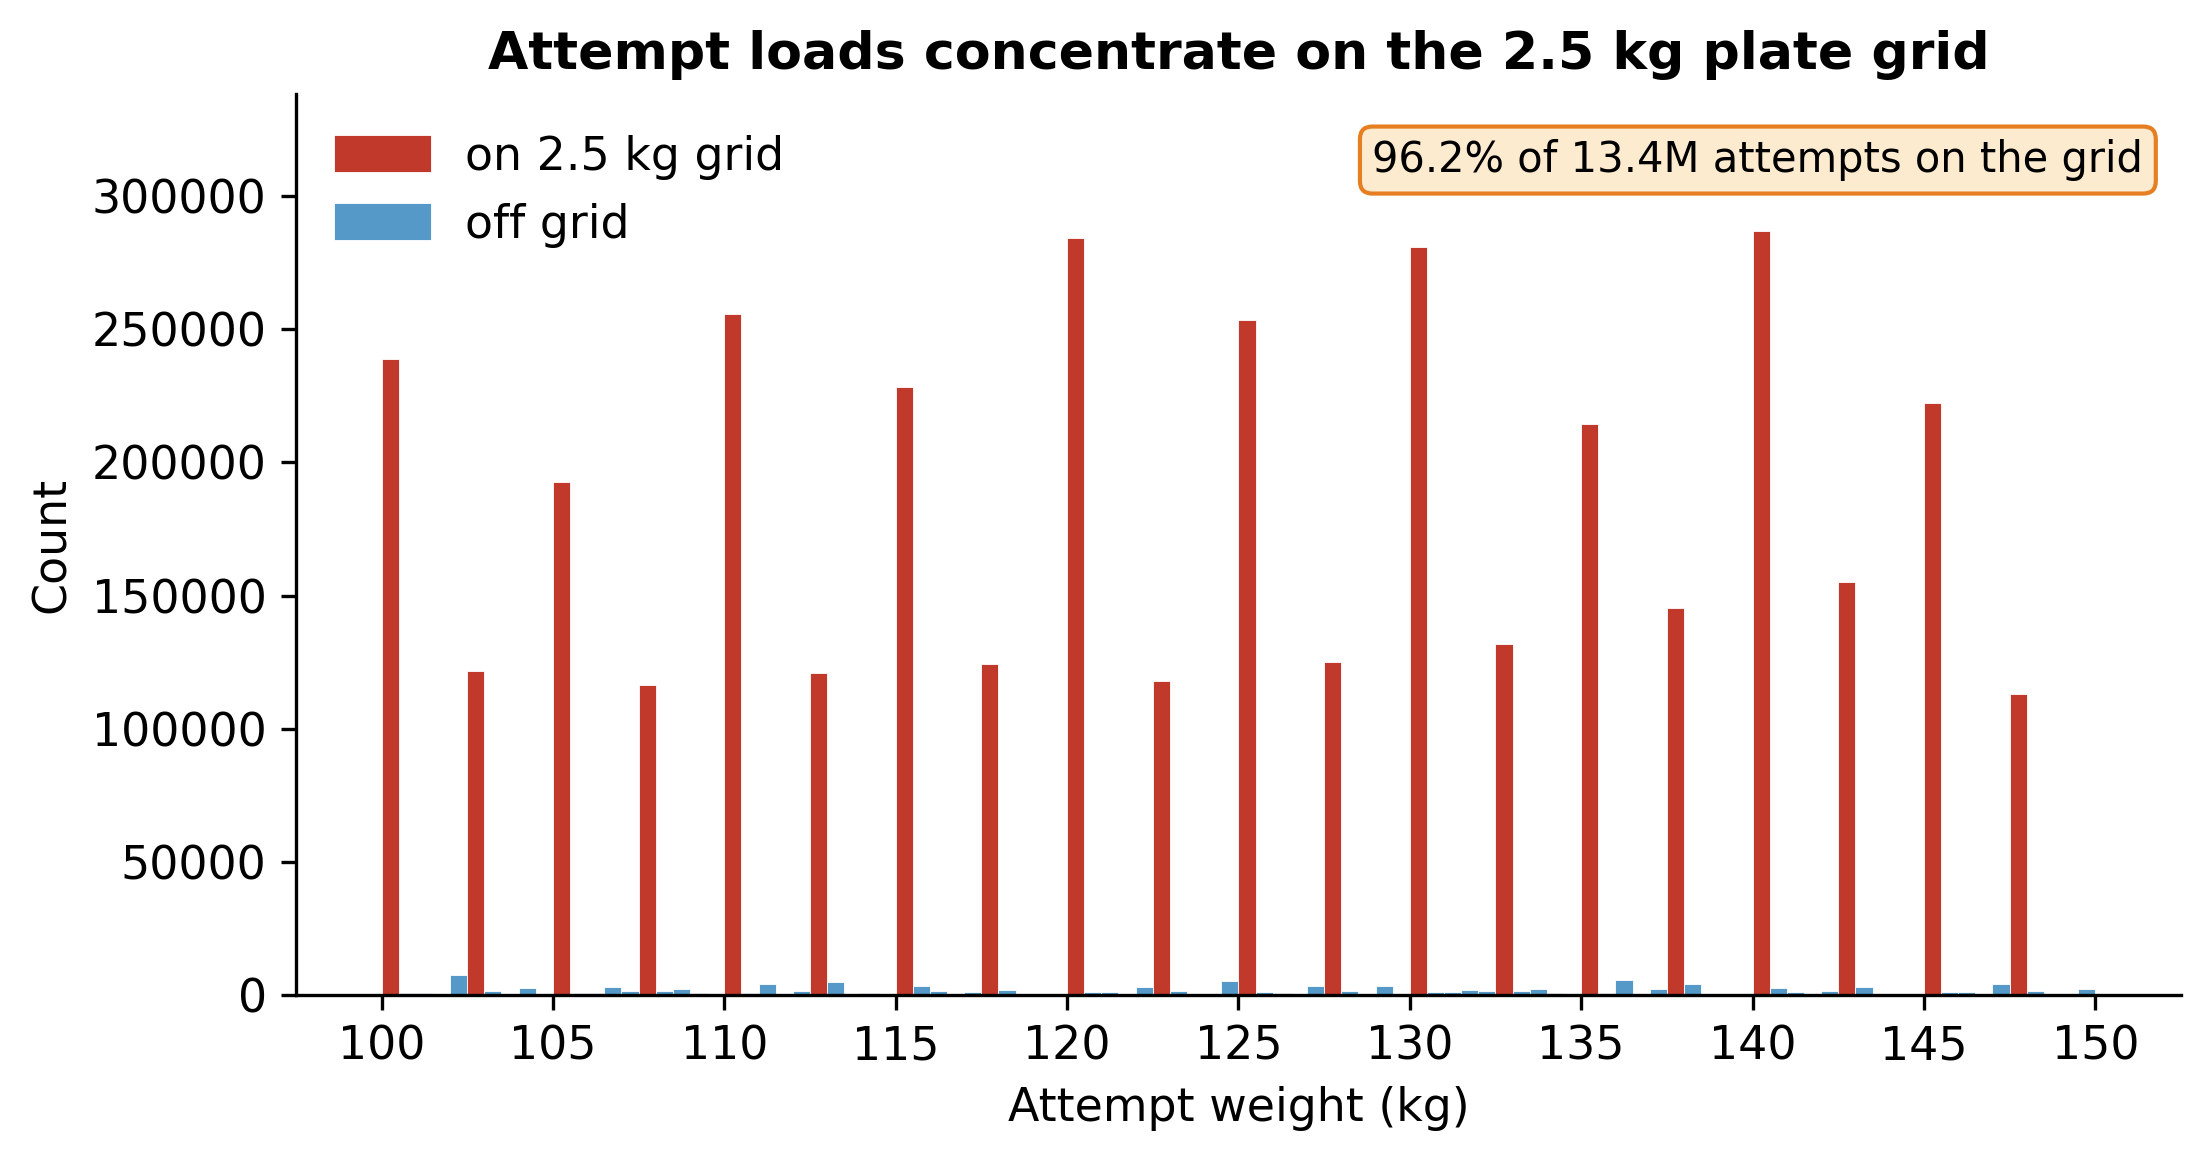
\includegraphics[width=\columnwidth]{fig1_quantization.png}
\caption{H1: attempt loads concentrate on the 2.5~kg plate grid.}
\label{fig:grid}\end{figure}

\subsection{Bodyweight bunches below class limits (H2)}
Bodyweight piles up just below real class limits (Fig.~\ref{fig:bunch}). On
de-heaped data (exact round/half-kg weigh-ins removed, so the signal is not mere
digit preference), the log-ratio of just-below to just-above counts is positive at
all seven IPF men's limits and strongest at 83~kg ($+1.92\pm0.04$, a $6.8\times$
asymmetry; Table~\ref{tab:limits}, Fig.~\ref{fig:limits}); a non-limit control at
91~kg is flat-to-slightly-negative ($-0.21$). The formal Cattaneo--Jansson--Ma
density-discontinuity test~\cite{cjm} (one random meet per lifter, de-heaped,
2014$+$) rejects at six of the seven limits with the density dropping at the cutoff
($t<0$), surviving both Holm and Benjamini--Hochberg correction; the lone exception
is the 120~kg cutoff ($t=-1.6$, $p=0.11$), adjacent to the unbounded $120{+}$ class
where the incentive to cut is weakest. The control shows no excess below (a small
\emph{opposite}-direction discontinuity), and no placebo shows the bunching
pattern. The effect is robust across equipment (raw $+2.14$, equipped $+1.51$) and
tested status (tested $+1.93$), and persists on the clean kg-only subset
($+1.80$).

\textbf{Robustness and falsification.} The result survives four checks. (i)~\emph{De-heaping}: removing exact round/half-kg weigh-ins leaves the
asymmetry intact, so the signal is not digit preference and is consistent with
weight-cut manipulation. (ii)~\emph{Control}:
the non-limit point at 91~kg shows no excess below. (iii)~\emph{Placebos}: cutoffs
placed between real limits show no bunching-direction discontinuity after
correction. (iv)~\emph{Subgroups and correction}: the effect holds within raw,
equipped, and tested subsets, and the formal density test rejects at six of the
seven limits even under the strictest (Bonferroni) correction.

\begin{figure*}[t]\centering
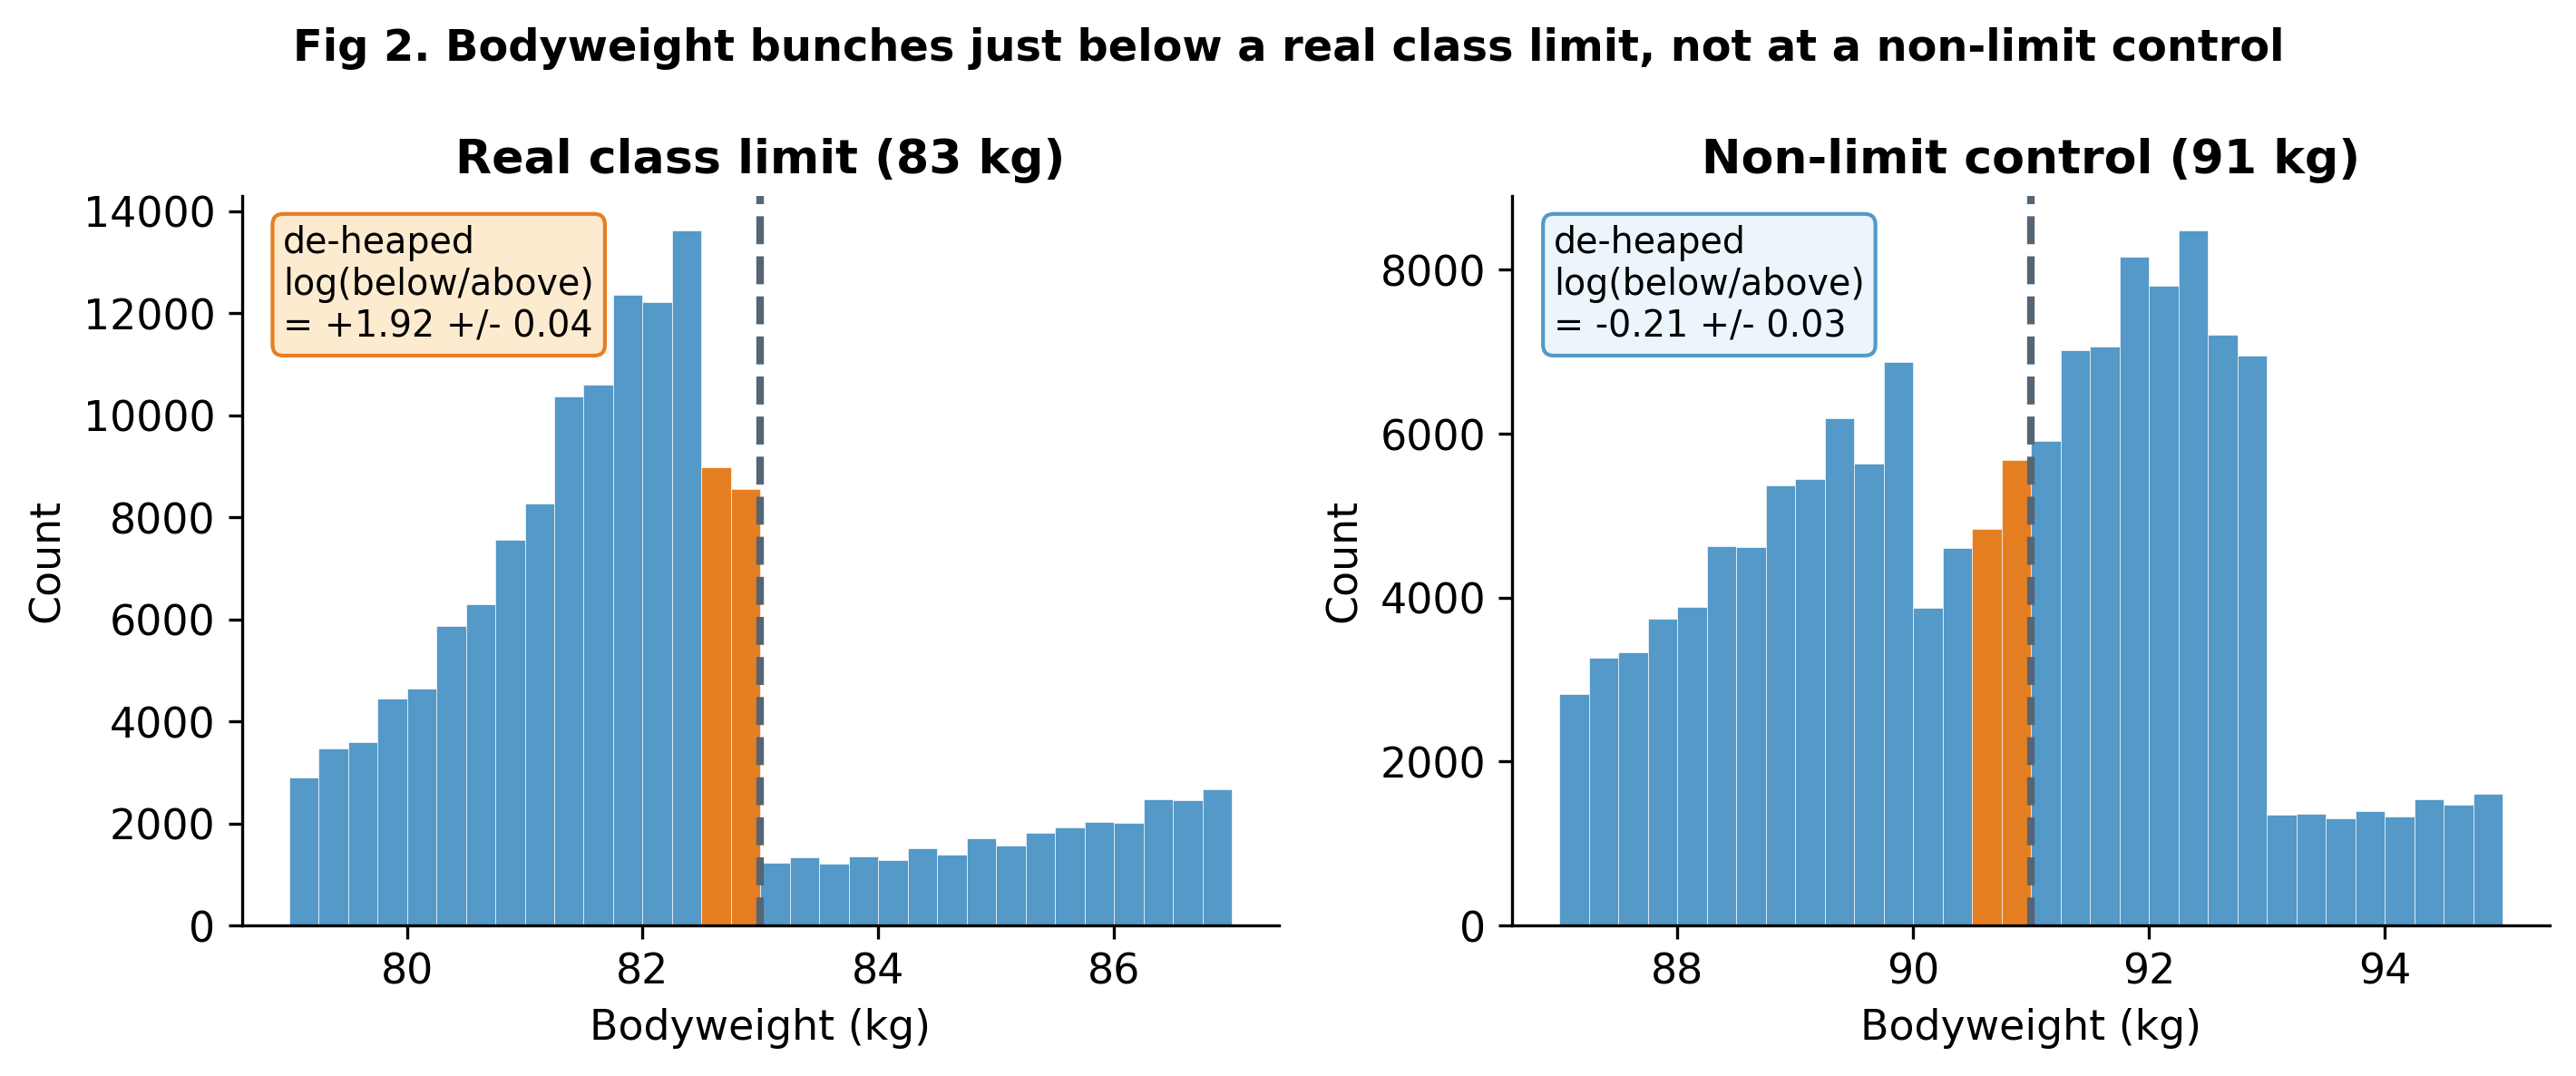
\includegraphics[width=0.86\textwidth]{fig2_bunching.png}
\caption{H2: bunching just below a real limit (83~kg) but not at a non-limit
control (91~kg); round-number weigh-ins removed.}
\label{fig:bunch}\end{figure*}

\begin{table}[t]\centering
\caption{De-heaped $\log(\text{below}/\text{above})$ at each IPF men's limit
(all rows). Last row is a non-limit control.}
\label{tab:limits}
\begin{tabular}{lccc}
\toprule
Limit (kg) & log-ratio & $\pm$ & $\times$ asymmetry\\
\midrule
59 & $+0.99$ & 0.04 & 2.7\\
66 & $+1.18$ & 0.03 & 3.2\\
74 & $+1.00$ & 0.03 & 2.7\\
\textbf{83} & $\mathbf{+1.92}$ & 0.04 & \textbf{6.8}\\
93 & $+1.65$ & 0.04 & 5.2\\
105 & $+1.17$ & 0.04 & 3.2\\
120 & $+0.74$ & 0.06 & 2.1\\
\midrule
91 (control) & $-0.21$ & 0.03 & 0.8\\
\bottomrule
\end{tabular}
\end{table}

\begin{figure}[t]\centering
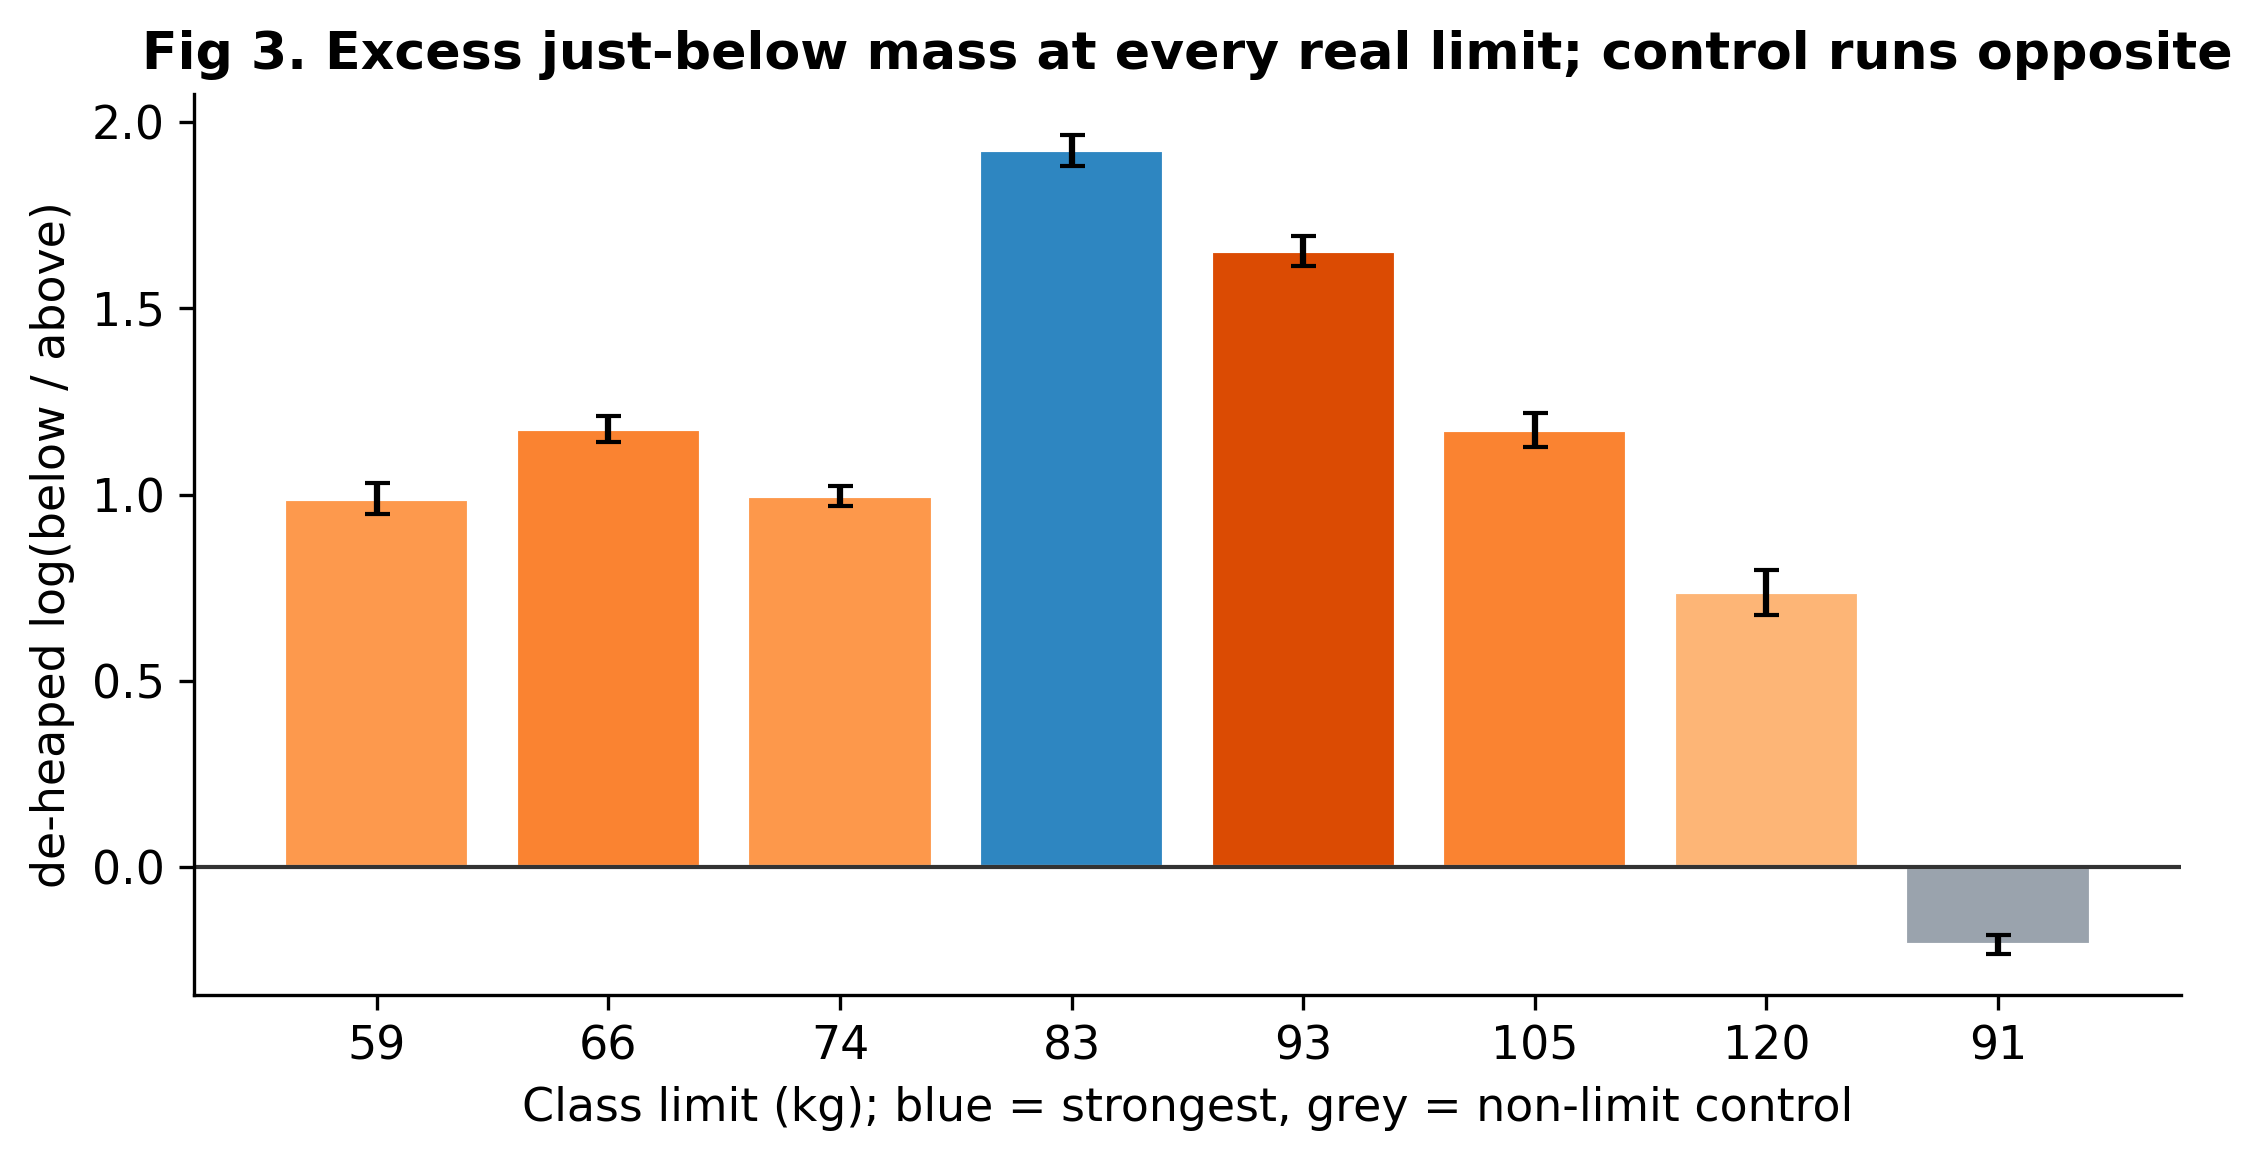
\includegraphics[width=\columnwidth]{fig3_all_limits.png}
\caption{H2: excess just-below mass at every real limit; control near zero.}
\label{fig:limits}\end{figure}

\subsection{Allometric scaling differs by sex (H3)}
Fitting $\log(\text{Total})=a+b\log(\text{BW})$ (Fig.~\ref{fig:allo}), the exponent
is $b=0.75$ (CI $[0.74,0.75]$) for men and $0.51$ ($[0.50,0.51]$) for women, with
heteroskedasticity-robust (HC3) standard errors on one row per lifter. A two-sided
Wald test rejects the isometric $b=2/3$ for both sexes, and in \emph{opposite}
directions (men $z=+46.8$, i.e.\ $b>2/3$; women $z=-64.1$, i.e.\ $b<2/3$). A pooled Sex$\times\log$(BW) interaction
estimates the men-minus-women slope gap at $+0.24$ ($p\!\ll\!10^{-3}$). The gap also \emph{grows} on the common bodyweight support ($0.84$ men vs.\ $0.38$
women), so it is not an artifact of the sexes occupying different weight ranges.
For men, the Pearson correlation of $\log\text{BW}$ and $\log\text{Total}$ is
$0.60$ (Fisher-transform CI $[0.60,0.603]$; Spearman $0.58$); it is lower for women. The message is not that women
are weaker, but that the \emph{estimated scaling} differs; we leave the mechanism to future
work.

\begin{figure}[t]\centering
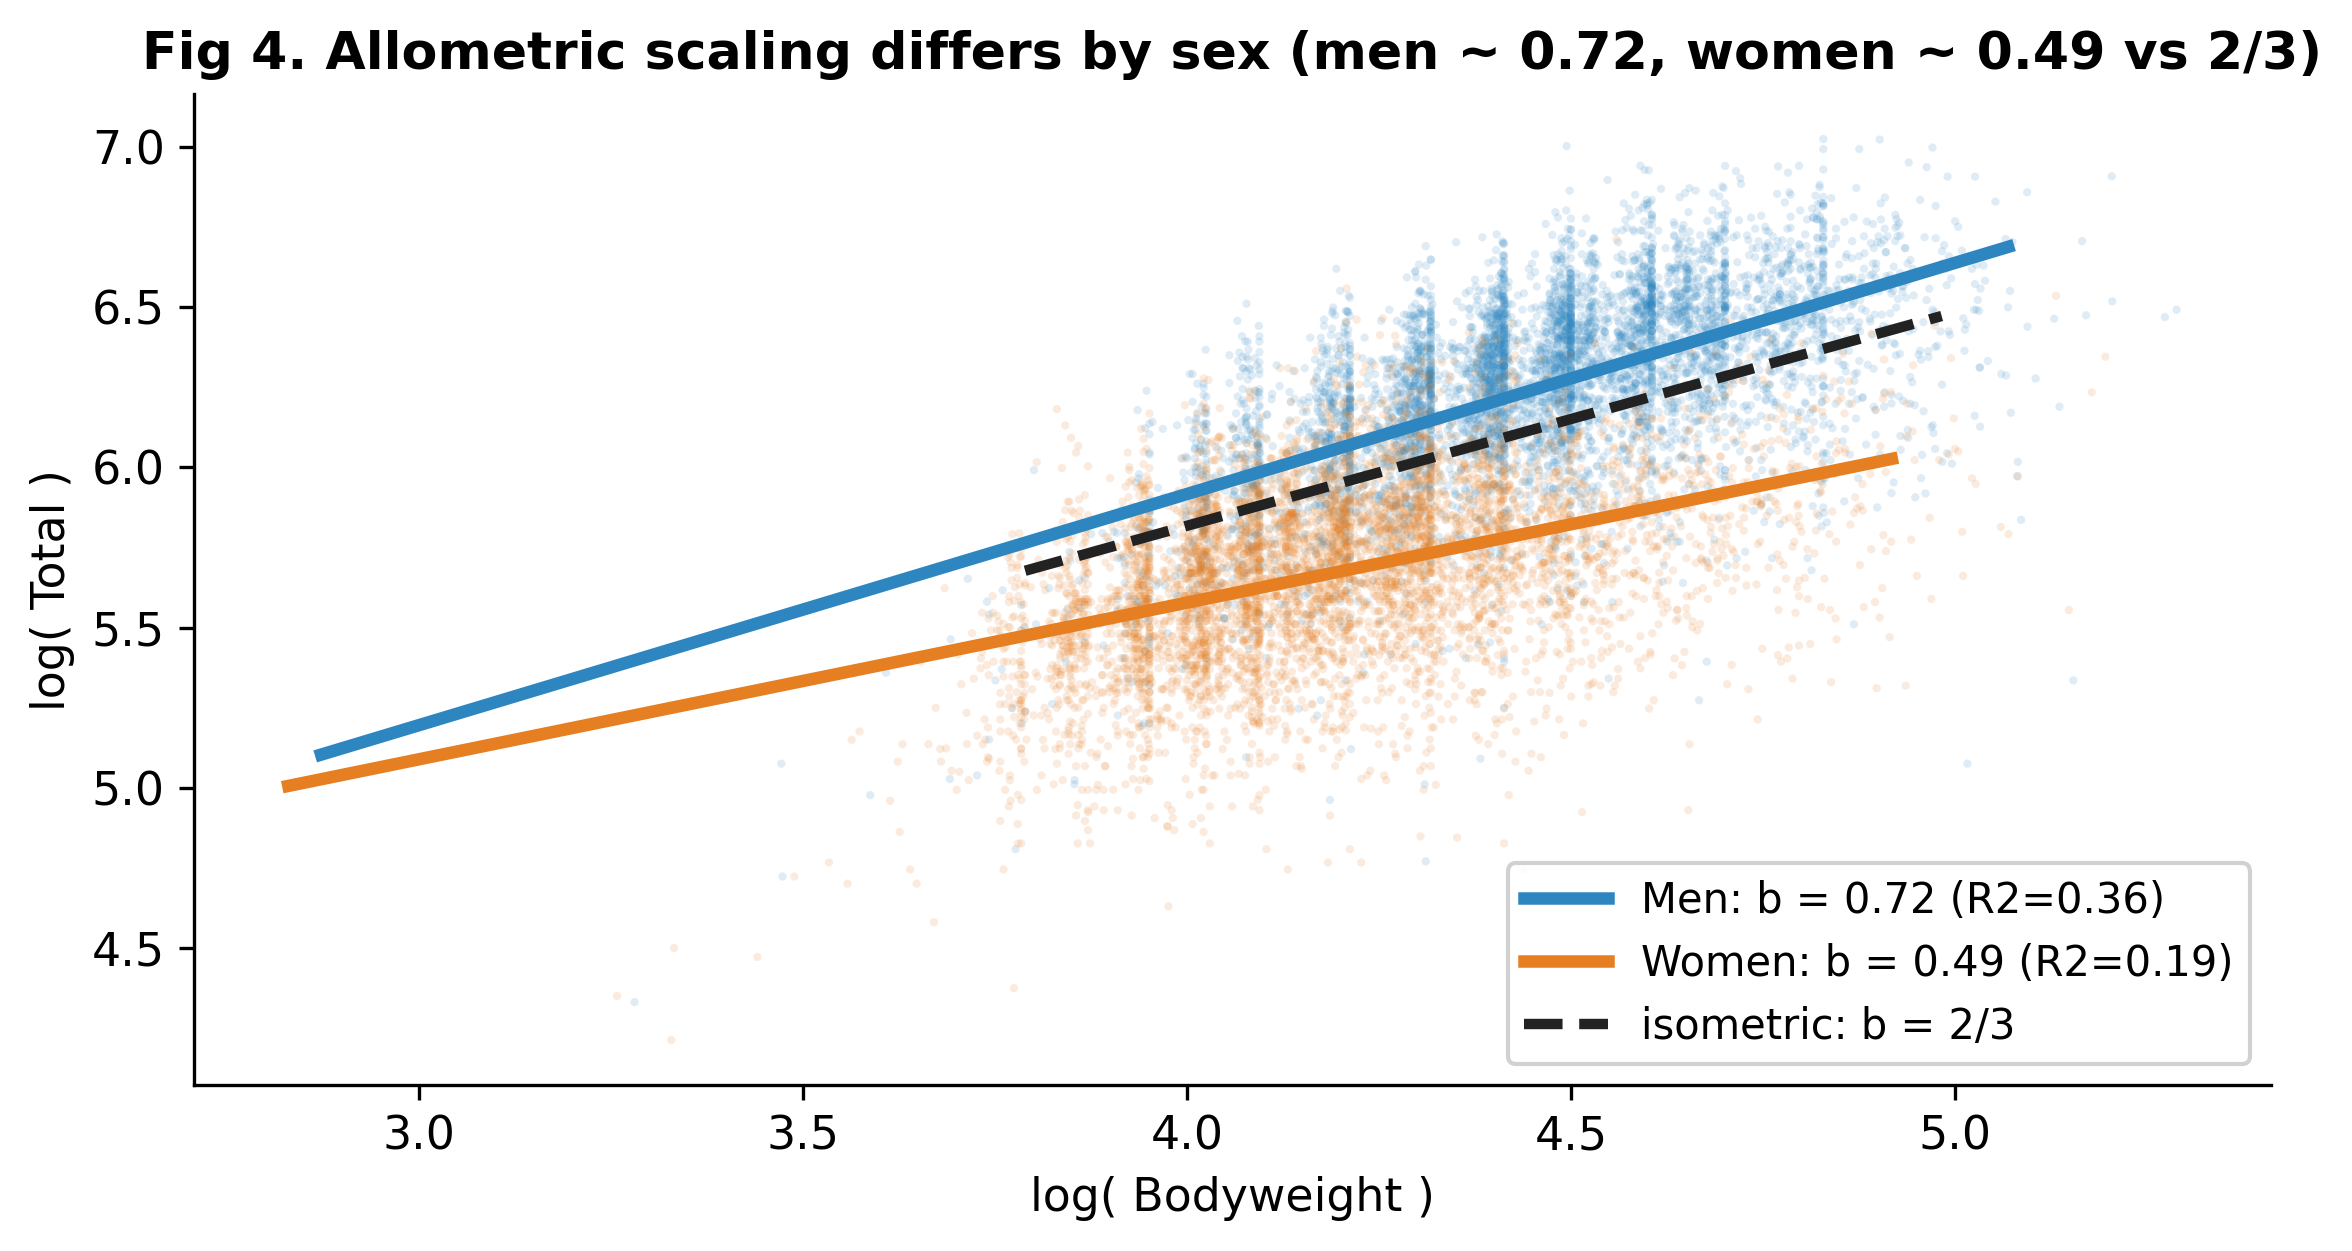
\includegraphics[width=\columnwidth]{fig4_allometry.png}
\caption{H3: allometric scaling by sex vs.\ the isometric $2/3$. Plotted lines are
all-row OLS fits; the headline per-lifter HC3 exponents are $0.75$ (men) / $0.51$ (women).}
\label{fig:allo}\end{figure}

\subsection{Strength is predictable from basic variables (H4)}
Predicting the total from controllable/basic variables (bodyweight, sex, equipment,
age), with every split grouped by lifter and all preprocessing fit inside each
training fold, a random forest reaches $R^2=0.70$ (RMSE $86$~kg) versus $0.61$
(RMSE $98$~kg) for linear regression (Fig.~\ref{fig:pred}); permutation importance
is dominated by sex and bodyweight, and continuous-feature VIFs are $\approx1$
(no collinearity concern). A logistic ``made-weight'' classifier built from
\emph{non-bodyweight} features (age, tested status, era, equipment; the Dots
score is excluded because it is a function of total and bodyweight) reaches
$\mathrm{AUC}=0.56$ (PR-AUC $0.84$, balanced accuracy $0.53$). The signal is weak,
as expected: cutting is driven by bodyweight relative to the limit, which defines
the label and which these features omit.

\begin{figure*}[t]\centering
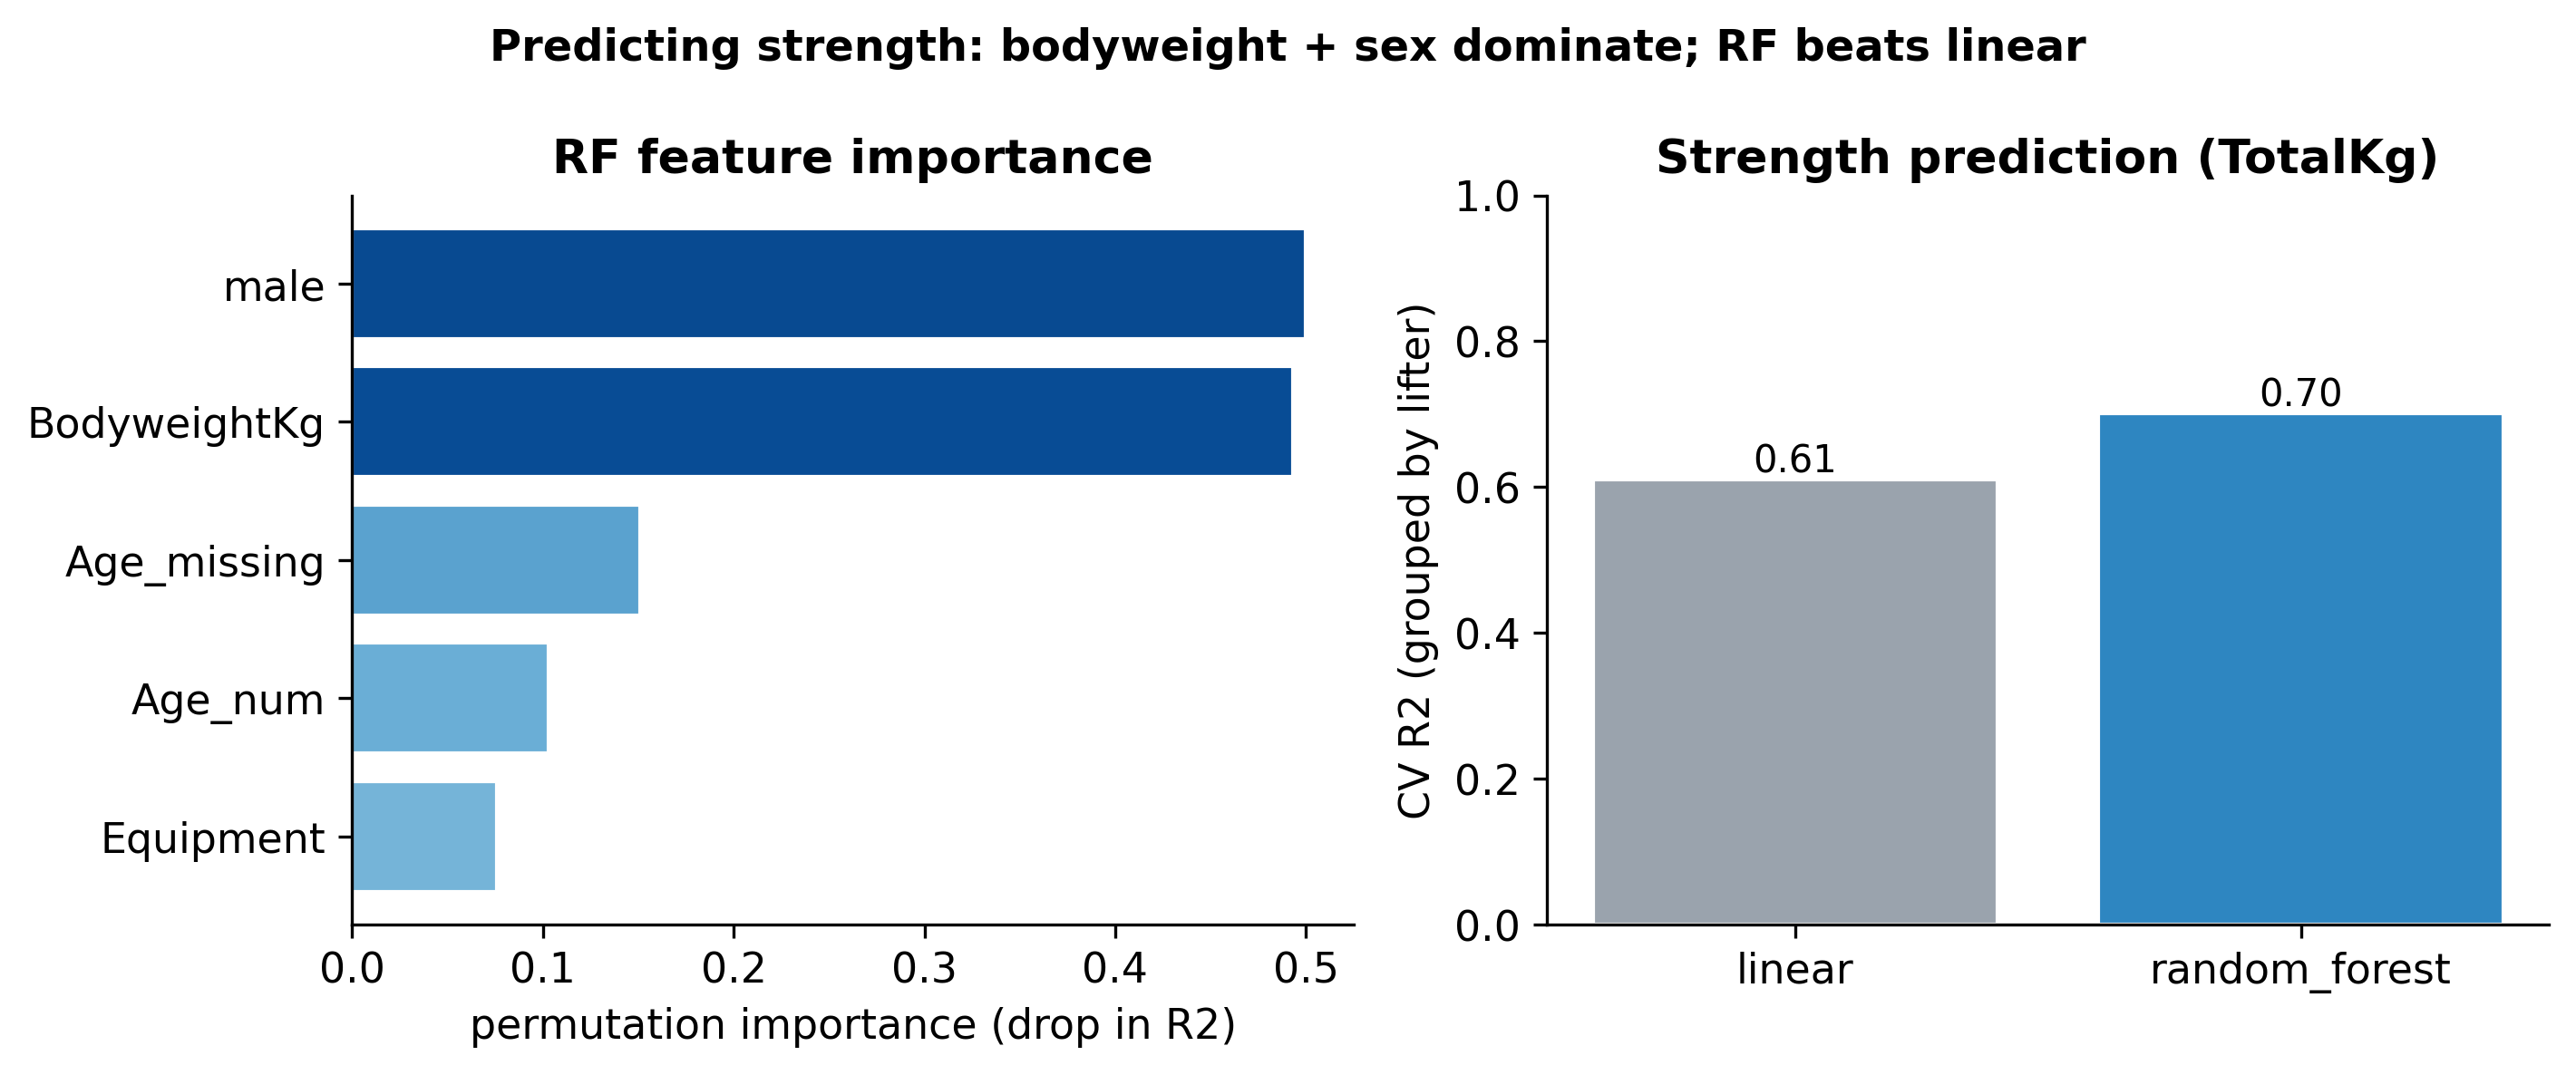
\includegraphics[width=0.86\textwidth]{fig5_prediction.png}
\caption{H4: strength prediction; importance and grouped-CV $R^2$.}
\label{fig:pred}\end{figure*}

\subsection{Supporting analyses}
\textbf{Distribution structure.} The apparent two-component shape of raw totals is
just sex: by BIC and a bootstrap likelihood-ratio test, raw Total prefers two
Gaussian components ($\Delta\mathrm{BIC}=1.4\times10^3$) but the sex-normalized
Dots score prefers one (Fig.~\ref{fig:struct}); the two-component shape largely
disappears after Dots normalization. \textbf{Tested vs.\ untested.} Untested competitions show
higher Dots than tested ones (medians $344$ vs.\ $318$, Mann--Whitney $p\!\to\!0$,
rank-biserial $-0.20$), consistent with---though not proof of---an effect of
performance-enhancing drugs, since tested and untested federations also differ in
era, equipment, and selection. \textbf{Extreme values.} A GEV fit to equal-size block maxima of recent
totals gives shape $\xi=-0.02$ with bootstrap CI $[-0.20,3.77]$: a population
strength \emph{ceiling is not supported}, since the CI includes zero. \textbf{Time
trend.} Median Dots drifted down over 2000--2024 (Spearman $\rho=-0.54$),
one possible explanation is broadening participation; the trend is not by itself
evidence of declining strength.
\textbf{Sequential detection.} A Wald sequential probability ratio test on the
chronological stream of just-below/above indicators accepts the bunching hypothesis
after a stopping time of only $N=27$ (Fig.~\ref{fig:breadth}). \textbf{Independence.}
After deduplicating to one row per lifter, the association between tested status and
cutting is negligible (Cram\'er's $V=0.008$), illustrating how pseudo-replication
inflates significance. \textbf{Residual normality.} The H3 (all-row fit) residuals are left-skewed
with a heavy lower tail (skew $-0.77$; Fig.~\ref{fig:norm}), so they are not exactly
normal. This does not undermine the slope: at this $n$ its sampling distribution is
asymptotically normal under standard conditions, and we report HC3-robust
standard errors. A formal normality test rejects even in modest subsamples
($n\!\approx\!300$), as expected for genuinely non-normal residuals, so we treat it
as a diagnostic and lead with effect sizes.

\begin{figure*}[t]\centering
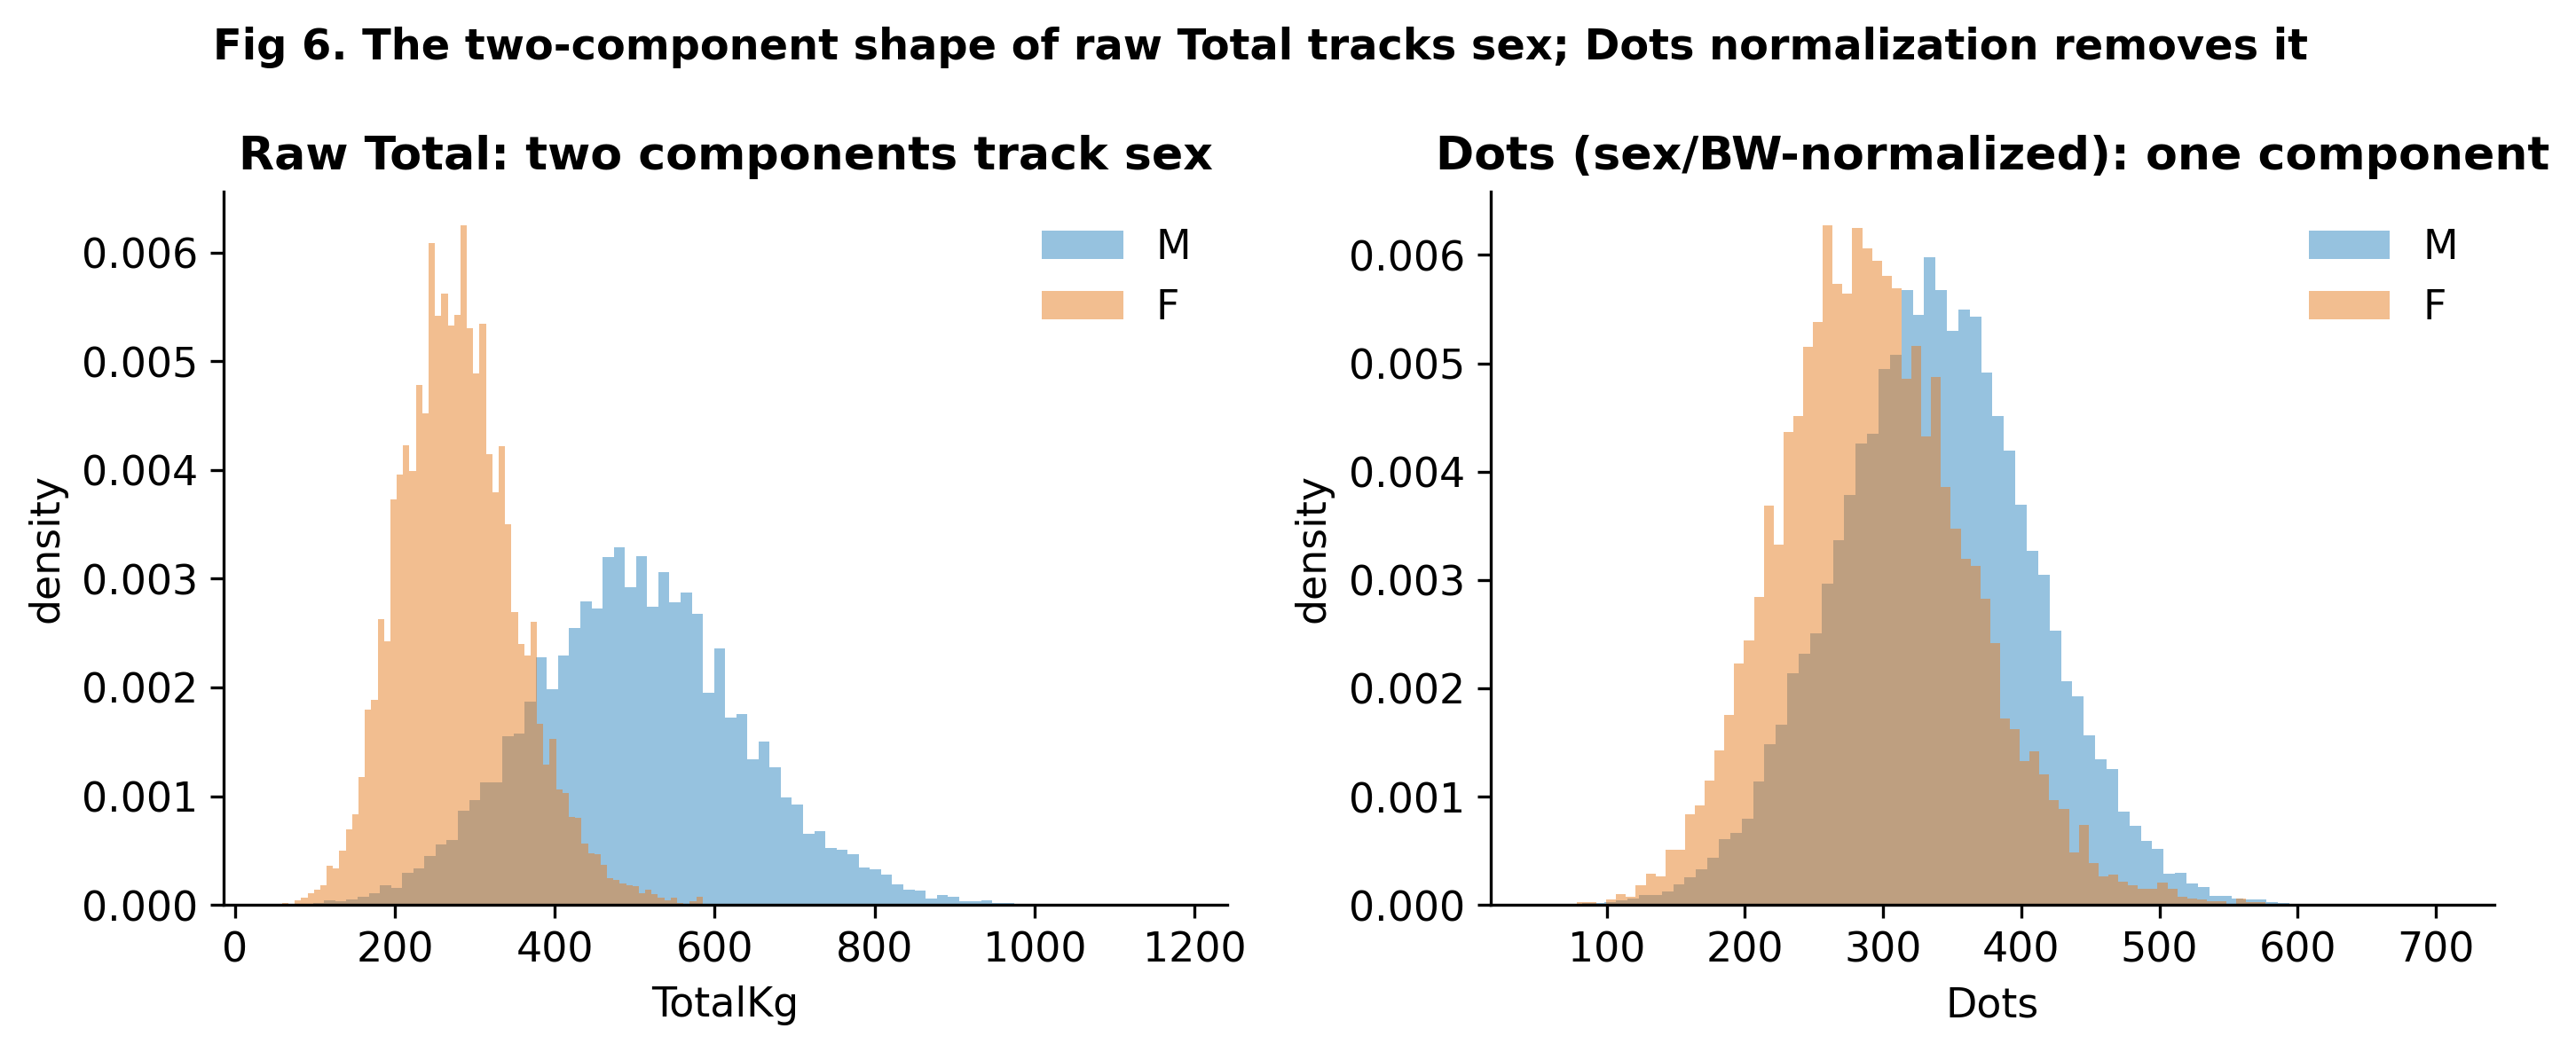
\includegraphics[width=0.86\textwidth]{fig6_structure.png}
\caption{The apparent ``mixture'' in raw Total is sex; Dots removes it.}
\label{fig:struct}\end{figure*}

\begin{figure*}[t]\centering
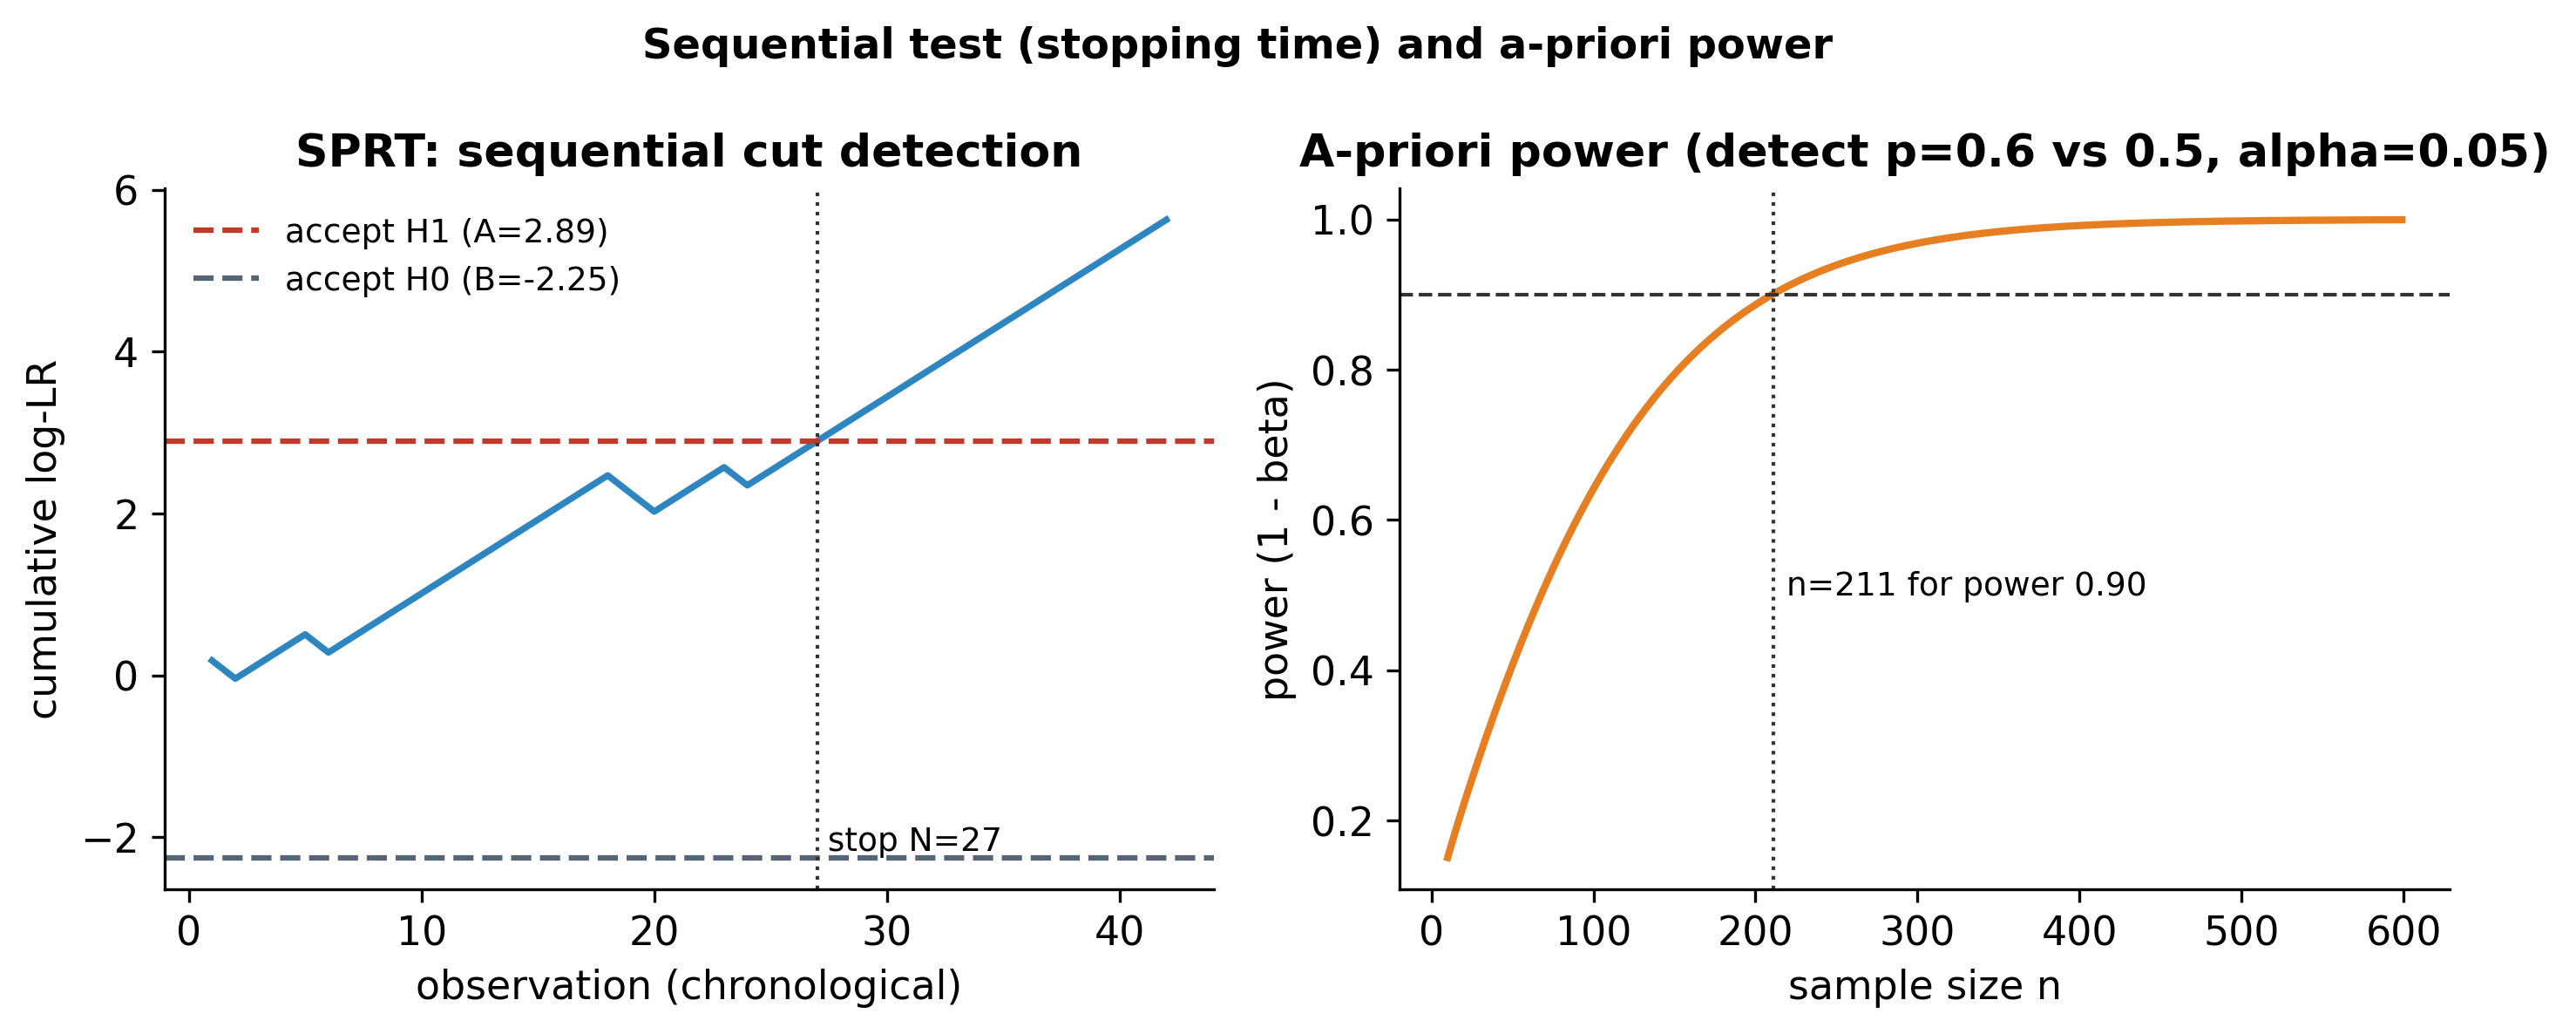
\includegraphics[width=0.86\textwidth]{fig7_breadth.png}
\caption{Sequential test (stopping time $N=27$) and a-priori power
($n=211$ for power $0.90$).}
\label{fig:breadth}\end{figure*}

\begin{figure*}[t]\centering
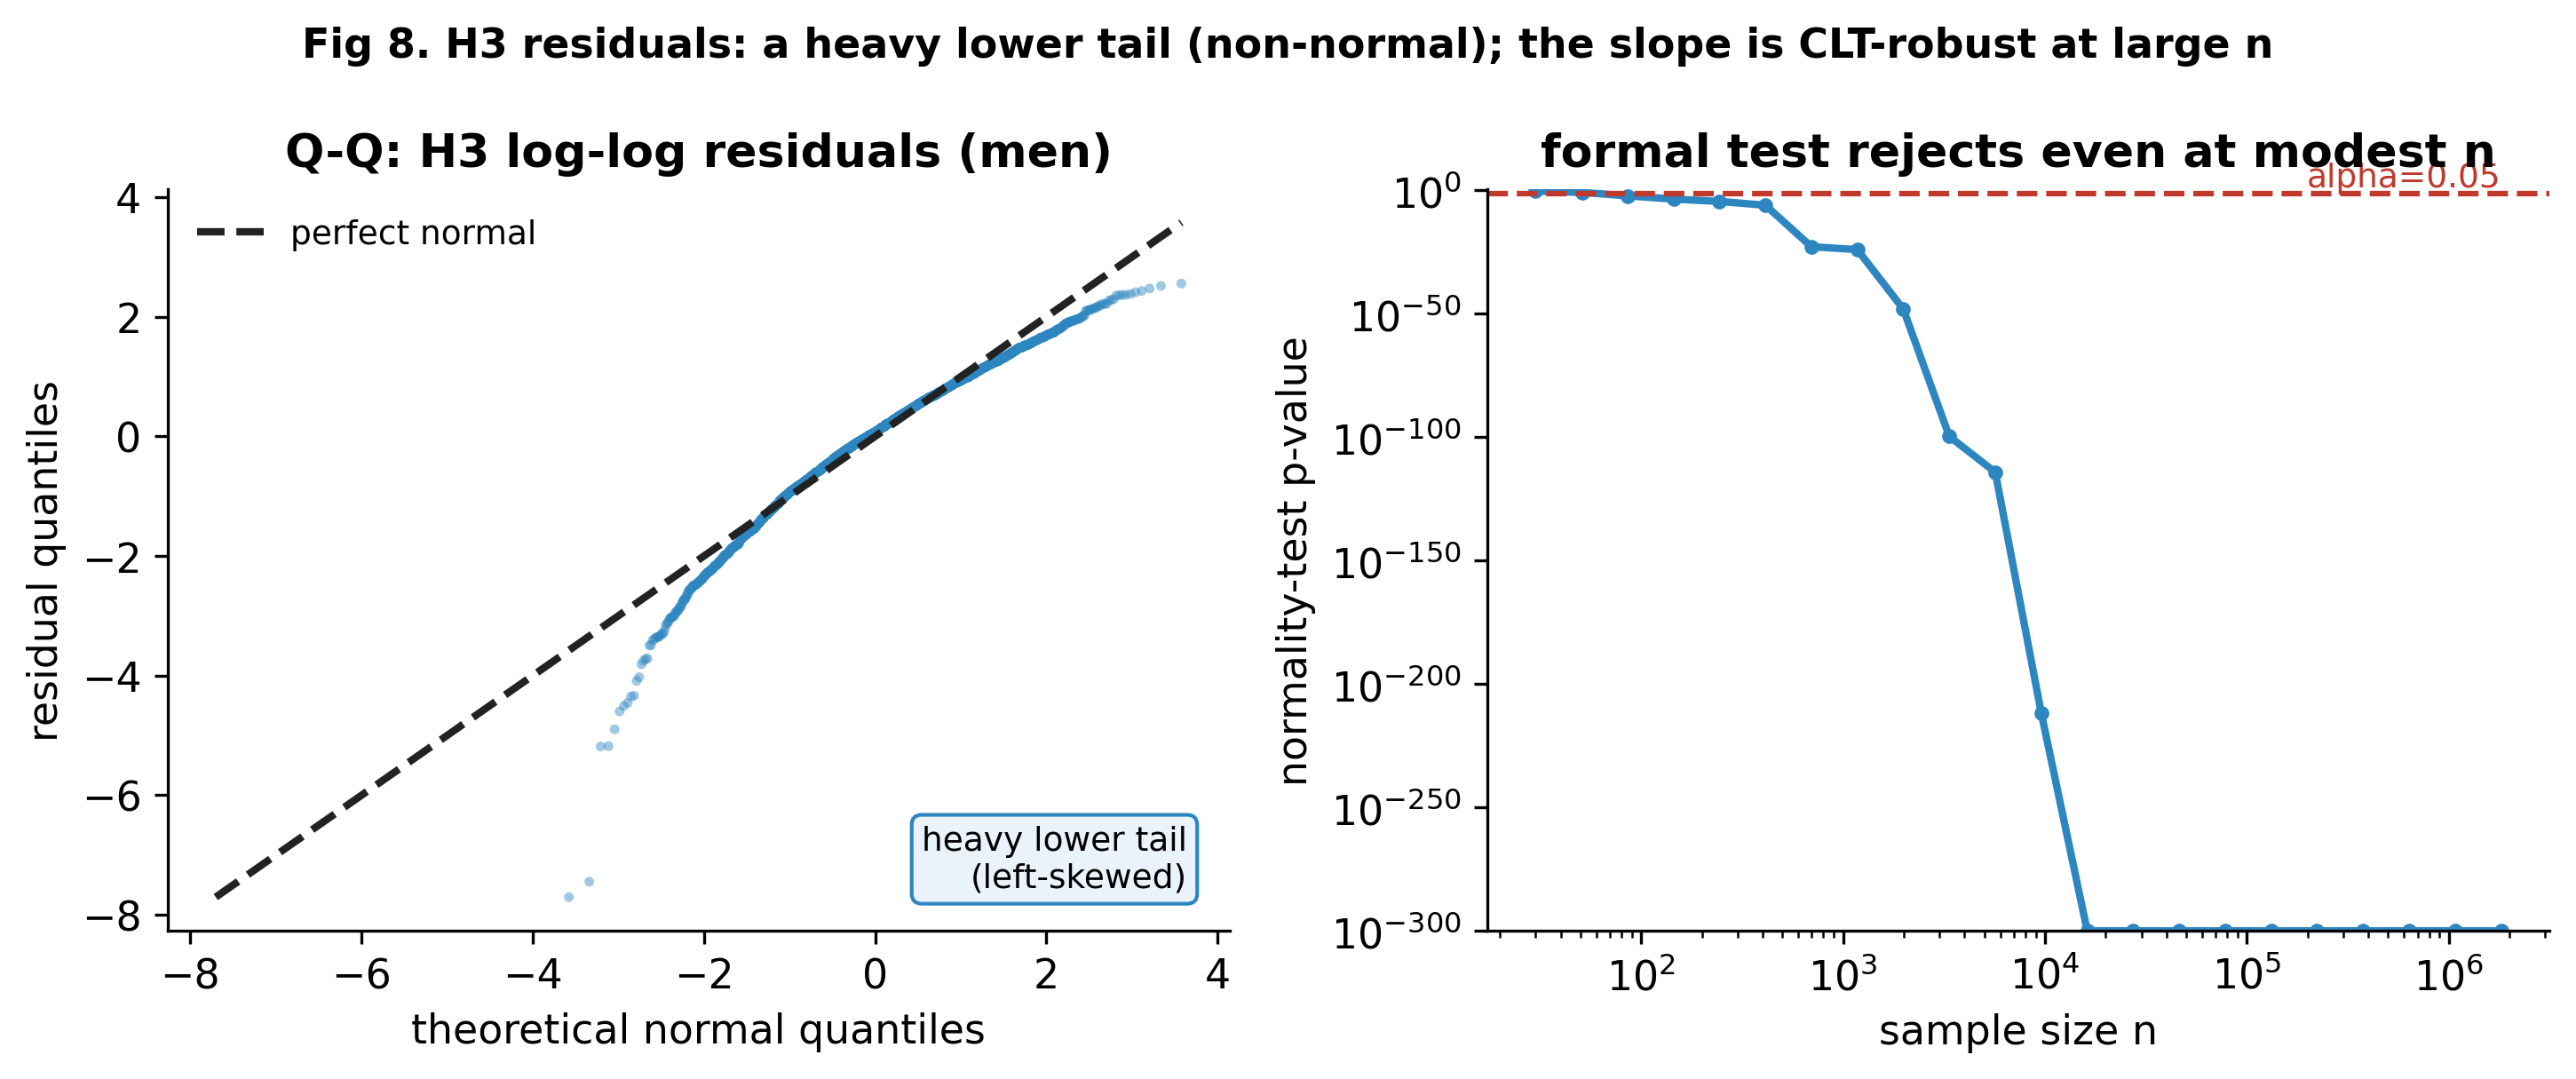
\includegraphics[width=0.86\textwidth]{fig8_normality.png}
\caption{H3 residuals: heavy lower tail; the slope is CLT-robust at large $n$.}
\label{fig:norm}\end{figure*}

\section{Methods}
\textbf{Data and preprocessing.} We use a pinned snapshot of OpenPowerlifting
(3{,}941{,}811 rows, public domain; the SHA-256 is recorded for exact
reproducibility). The unit of analysis is the \emph{attempt} for H1 (the mechanism
is within-competitor, so the grid is robust to clustering) and one \emph{row per
lifter} for the cross-sectional tests; \emph{de-heaping} drops exact round/half-kg
weigh-ins so the bunching signal is not digit preference. For prediction, all cross-%
validation is grouped by lifter so the same athlete never appears in both train and
test.

\textbf{GLRT and the boundary (H1).} With log-likelihood $\ell$, the statistic is
$2\ln\Lambda=2(\ell_1-\ell_0)$. Under regularity $2\ln\Lambda\to\chi^2_{r}$, but
when the null fixes a parameter on the boundary of its space the limit becomes a
mixture $\tfrac12\chi^2_0+\tfrac12\chi^2_1$~\cite{chernoff,selfliang}; we estimate
the null distribution directly by simulating data under the fitted null model
(parametric bootstrap) and comparing the observed statistic to the simulated
quantiles. Concretely, for within-cell position $u\in\{0,\dots,4\}$ on the 0.5~kg
lattice the model is
\begin{equation}
P(u)=\pi\,\mathbb{1}[u=0]+(1-\pi)\tfrac15,\qquad \pi\in[0,1],
\end{equation}
and the GLRT contrasts $\pi=0$ (no grid preference, on the boundary) with the
constrained MLE $\hat\pi\ge0$.

\textbf{Density discontinuity (H2).} For a cutoff $c$ the manipulation test
contrasts the one-sided densities, $\theta=\ln \hat f^{+}(c)-\ln \hat f^{-}(c)$,
estimated by local polynomials without pre-binning~\cite{mccrary,cjm}; $\theta<0$
($t<0$) indicates excess mass just below $c$. We complement the formal test with a
de-heaped log count-ratio as the interpretable effect size.

\textbf{Allometry (H3).} OLS on $\log$--$\log$ data gives the scaling exponent
$b$; we report HC3-robust standard errors (one row per lifter), a Wald statistic
$W=(\hat b-2/3)/\widehat{\mathrm{se}}(\hat b)$, and a pooled
Sex$\times\log$(BW) interaction whose coefficient is exactly the men-minus-women
slope difference. Correlations use the Fisher $z$-transform for confidence
intervals.

\textbf{Learning and the rest of the toolbox.} Prediction uses linear and
random-forest regression and logistic classification, evaluated by grouped
cross-validation ($R^2$, adjusted $R^2$, RMSE, MAE, permutation importance, VIF,
AUC/PR-AUC). Supporting analyses use a bootstrap mixture-LRT with AIC/BIC, a GEV
extreme-value fit, a Wald sequential probability ratio test (with decision
boundaries $A=\ln\frac{1-\beta}{\alpha}$, $B=\ln\frac{\beta}{1-\alpha}$, a stopping
time, and an expected-sample-size approximation), one- and two-sample nonparametric
tests (Wilcoxon signed-rank; Mann--Whitney), an $F$-test/Kruskal--Wallis omnibus
with post-hoc comparisons, and a $\chi^2$ independence test with Cram\'er's $V$ and
standardized residuals. The extreme-value fit uses the GEV distribution
\begin{equation}
G(x)=\exp\!\Big\{-\big(1+\xi\tfrac{x-\mu}{\sigma}\big)^{-1/\xi}\Big\},
\end{equation}
where $\xi<0$ implies a bounded upper tail (a strength ceiling) and $\xi\ge0$ does
not; we estimate $\xi$ from equal-size block maxima and bootstrap its interval. The
sequential test's expected sample size under the alternative is approximated by
$\mathbb{E}[N\mid H_1]\approx\big[(1-\beta)A+\beta B\big]/\big[p_1 s_1+(1-p_1)s_0\big]$,
with $s_0,s_1$ the per-observation log-likelihood increments.
Table~\ref{tab:tools} maps the course toolbox onto the study.

\textbf{Reproducibility.} Every result is produced by a small set of scripts from
the pinned snapshot; numbers are written to machine-readable files, figures are
exported at 300~DPI, and an independent re-derivation from the raw data reproduced
every headline value reported here.

\begin{table}[t]\centering
\caption{Coverage of the course toolbox.}
\label{tab:tools}
\begin{tabular}{ll}
\toprule
Concept & Where used\\
\midrule
GLRT, MLE, $\chi^2$ goodness-of-fit & H1 grid model\\
Boundary LRT, parametric bootstrap & H1 null calibration\\
Density discontinuity (McCrary/CJM) & H2 bunching\\
Multiple testing (Bonf./Holm/\v{S}id\'ak/BH) & H2 limits, H3\\
OLS, $R^2$, Wald, interaction term & H3 allometry\\
One-/two-sided, one-sample tests & H1, H3\\
Pearson/Spearman, Fisher CI & H3\\
Regression, random forest, logistic & H4 prediction\\
Learning metrics, grouped CV, VIF & H4\\
Mixture LRT, AIC/BIC & structure\\
Mann--Whitney (two-sample) & tested vs.\ untested\\
Wilcoxon signed-rank (paired) & attempt 1 vs.\ 3\\
$F$/ANOVA, Kruskal--Wallis, post-hoc & equipment\\
$\chi^2$ independence, Cram\'er's $V$ & tested $\times$ cut\\
Extreme-value theory (GEV) & strength ceiling\\
Sequential Wald (SPRT), stopping time & cut detection\\
Power, Type I/II tradeoff & a-priori power\\
\bottomrule
\end{tabular}
\end{table}

\section{Discussion}
\textbf{Conclusions.} The two numbers a competitor controls leave measurable,
falsification-surviving traces. Attempt loads are quantized to the plate grid;
bodyweight bunches specifically below class limits, and not at controls or placebos
in the bunching direction. Beyond strategy, the data also bear on the limits of
strength: scaling with bodyweight is sex-specific and departs from the isometric
$2/3$, and basic meet-record variables already explain $\sim$70\% of the variance
in the total. The same dataset supports the descriptive, testing, and prediction
analyses.

\textbf{Limitations and null results.} This is an observational study: we identify
population-level patterns consistent with weight cutting, not the intent of any
individual. We report three null results as genuine findings. The unbounded
$120{+}$ class does \emph{not} show significant bunching after correction
($t=-1.6$, $p=0.11$), consistent with weaker cutting pressure at that open-ended
boundary; the extreme-value analysis does \emph{not} support a strength ceiling
(the $\xi$ confidence interval includes zero); and we find no material association
between tested status and cutting once pseudo-replication is removed. On the methods side,
lifter identity is name-based, the per-lifter meet is sampled at random, and the
formal bunching test is restricted to the modern kg-only era. The 83~kg signal is
robust to the federation set: the de-heaped log-ratio is $+1.92$ across the
IPF-affiliated federations used here and $+1.66$ when restricted to IPF/USAPL alone.
Several extensions remain for future work: more federations and eras, a
structural bunching model that recovers the share of manipulators, and a
multiverse robustness check.

\begin{thebibliography}{9}
\bibitem{kleven} H.~J.~Kleven, ``Bunching,'' \emph{Annual Review of Economics},
vol.~8, pp.~435--464, 2016.
\bibitem{mccrary} J.~McCrary, ``Manipulation of the running variable in the
regression discontinuity design: A density test,'' \emph{J.\ Econometrics},
vol.~142, no.~2, pp.~698--714, 2008.
\bibitem{cjm} M.~D.~Cattaneo, M.~Jansson, and X.~Ma, ``Simple local polynomial
density estimators,'' \emph{J.\ Amer.\ Statist.\ Assoc.}, vol.~115, no.~531,
pp.~1449--1455, 2020.
\bibitem{chernoff} H.~Chernoff, ``On the distribution of the likelihood ratio,''
\emph{Ann.\ Math.\ Statist.}, vol.~25, no.~3, pp.~573--578, 1954.
\bibitem{selfliang} S.~G.~Self and K.-Y.~Liang, ``Asymptotic properties of maximum
likelihood estimators and likelihood ratio tests under nonstandard conditions,''
\emph{J.\ Amer.\ Statist.\ Assoc.}, vol.~82, no.~398, pp.~605--610, 1987.
\bibitem{einmahl} J.~H.~J.~Einmahl and J.~R.~Magnus, ``Records in athletics through
extreme-value theory,'' \emph{J.\ Amer.\ Statist.\ Assoc.}, vol.~103, no.~484,
pp.~1382--1391, 2008.
\bibitem{peyen} Peyen \emph{et al.}, ``Discussing diminishing returns: A new
scoring system for powerlifting,'' arXiv:2503.13040, 2025.
\bibitem{opl} OpenPowerlifting, \url{https://www.openpowerlifting.org} (data
released into the public domain).
\end{thebibliography}

\end{document}
